\documentclass[9pt,aspectratio=169,xcolor=table]{beamer}

%~~~~~~~~~~~~~~~~~~~~~~~~~~~~~~~~~~~~~~~~~~~~~~~~~~~~~~~~~~~~~~~~~~~~~~~~~~~~~~
% Use roboto Font (recommended)
\usepackage[sfdefault]{roboto}
\usepackage[utf8]{inputenc}
\usepackage[T1]{fontenc}
%~~~~~~~~~~~~~~~~~~~~~~~~~~~~~~~~~~~~~~~~~~~~~~~~~~~~~~~~~~~~~~~~~~~~~~~~~~~~~~

%~~~~~~~~~~~~~~~~~~~~~~~~~~~~~~~~~~~~~~~~~~~~~~~~~~~~~~~~~~~~~~~~~~~~~~~~~~~~~~
% Define where theme files are located. ('/styles')
\usepackage{styles/fluxmacros}
\usefolder{styles}
% Use Flux theme v0.1 beta
% Available style: asphalt, blue, red, green, gray
\usetheme[style=hunter]{flux}
%~~~~~~~~~~~~~~~~~~~~~~~~~~~~~~~~~~~~~~~~~~~~~~~~~~~~~~~~~~~~~~~~~~~~~~~~~~~~~~

%~~~~~~~~~~~~~~~~~~~~~~~~~~~~~~~~~~~~~~~~~~~~~~~~~~~~~~~~~~~~~~~~~~~~~~~~~~~~~~
% Extra packages
\usepackage{booktabs}
\usepackage{colortbl}
\usepackage{ragged2e}
\usepackage{amssymb}
\usepackage{multirow}
\usepackage{tikz}
\usetikzlibrary{arrows.meta, positioning, fit, backgrounds, calc, decorations.pathreplacing}
\setbeamertemplate{itemize items}[square]
\usepackage[scaled=.8]{beramono}
\usepackage{listings}
\usepackage{styles/lstlangarm}
\usepackage{array}
\definecolor{bgcolor}{HTML}{F2E9E9}
% lstlangarm.sty references \color{mauve} for string literals but never defines
% it -- only fires when a listing contains a string. Define it here.
\definecolor{mauve}{rgb}{0.58,0,0.82}
% lstlangarm's C style sets commentstyle=green!20, which is unreadable on the
% pink listing background. Darken it globally.
\lstset{commentstyle=\color{green!45!black}}
% ragged-right fixed-width column -- must be defined in the preamble, never
% inside a frame (\newcolumntype's #1 breaks beamer's frame scanner)
\newcolumntype{R}[1]{>{\RaggedRight\arraybackslash}p{#1}}
%~~~~~~~~~~~~~~~~~~~~~~~~~~~~~~~~~~~~~~~~~~~~~~~~~~~~~~~~~~~~~~~~~~~~~~~~~~~~~~
% Table striping: odd rows white, even rows very light gray.
% Needs \documentclass[...,xcolor=table]{beamer} (beamer loads xcolor itself,
% so the option must go on the class, not \usepackage).
\definecolor{stripe}{gray}{0.94}
% \striped makes body rows alternate white, gray, white, ... starting white.
% \rowcolors counts from the first coloured body row; the header is not counted.
\newcommand{\striped}{\rowcolors{1}{white}{stripe}}
%~~~~~~~~~~~~~~~~~~~~~~~~~~~~~~~~~~~~~~~~~~~~~~~~~~~~~~~~~~~~~~~~~~~~~~~~~~~~~~

%~~~~~~~~~~~~~~~~~~~~~~~~~~~~~~~~~~~~~~~~~~~~~~~~~~~~~~~~~~~~~~~~~~~~~~~~~~~~~~
% TikZ block styles -- matches ch1/ch2
% Colour variables are named identically in the book's stm32primer.tex, so any
% tikzpicture using only the \tikzset{...} styles below can be copied verbatim
% between slides and book. Only the \definecolor/\colorlet VALUES differ: the
% book is printed, so it keeps every stroke pure black with muted fills. These
% slides are projected, so both fill AND stroke are bright and saturated to
% grab attention -- see stm32primer.tex for the print palette.
\definecolor{blkfill}{HTML}{DDEEDD}
\definecolor{blkline}{HTML}{355E3B}
\definecolor{accentfill}{HTML}{FFE0B2}
\definecolor{accentline}{HTML}{E65100}
\definecolor{memfill}{HTML}{DFF5DA}
\definecolor{memline}{HTML}{2E7D32}
\definecolor{cellfill}{HTML}{FFFFFF}
\definecolor{cellline}{HTML}{424242}
\definecolor{bitmaskfill}{HTML}{DCEBFF}
\definecolor{bitmaskline}{HTML}{1565C0}
\definecolor{bithitfill}{HTML}{FFE0B2}
\definecolor{bithitline}{HTML}{E65100}
\tikzset{
  blk/.style   = {rectangle, rounded corners=2pt, draw=blkline, fill=blkfill,
                  thick, align=center, font=\small, minimum height=9mm, inner sep=3pt},
  cpublk/.style= {rectangle, rounded corners=2pt, draw=accentline, fill=accentfill,
                  thick, align=center, font=\small\bfseries, minimum height=9mm, inner sep=3pt},
  memblk/.style= {rectangle, rounded corners=2pt, draw=memline, fill=memfill,
                  thick, align=center, font=\small, minimum height=9mm, inner sep=3pt},
  cell/.style  = {rectangle, draw=cellline, fill=cellfill, align=center,
                  font=\small\ttfamily, minimum height=7mm, inner sep=2pt},
  bitcell/.style={rectangle, draw=cellline, fill=cellfill, thick,
                  minimum width=5.4mm, minimum height=5.4mm, inner sep=0pt,
                  font=\scriptsize\ttfamily, anchor=center},
  bitmask/.style={bitcell, fill=bitmaskfill, draw=bitmaskline},
  bithit/.style ={bitcell, fill=bithitfill, draw=bithitline, font=\scriptsize\ttfamily\bfseries},
  rowlab/.style ={font=\scriptsize, text=Gray, anchor=east},
  oplab/.style  ={font=\scriptsize\itshape, text=Gray, anchor=west},
  lbl/.style   = {font=\scriptsize, text=Gray},
  flow/.style  = {-{Stealth[length=2mm]}, thick, draw=blkline},
  busline/.style={thick, draw=cellline},
}
% NOTE (theme quirks -- all fail SILENTLY, always page through the PDF):
%  - a second \\ inside a nested {...} group in a TikZ node breaks parsing
%  - {\small ...} wrapped around a nested itemize eats the frame title + list
%  - \usebeamercolor on a [plain] frame falls through to an unstyled default
%  - \newcolumntype inside a frame breaks beamer's frame scanner
%  - lstlisting needs \begin{frame}[fragile]
%  - a TikZ picture wider than its column silently overflows into neighbours
%~~~~~~~~~~~~~~~~~~~~~~~~~~~~~~~~~~~~~~~~~~~~~~~~~~~~~~~~~~~~~~~~~~~~~~~~~~~~~~

%%%%%%%%%%%%%%%%%%%%%%%%%%%%%%%%%%%
%% BEGIN CONDITIONAL COMPILATION %%
%%%%%%%%%%%%%%%%%%%%%%%%%%%%%%%%%%%
\newif\ifwebex
%\webextrue % uncomment to generate section separator
\ifwebex
\AtBeginSection[]{
  \begin{frame}
  \vfill
  \centering
  \begin{beamercolorbox}[sep=8pt,center,shadow=true,rounded=true]{title}
    \usebeamerfont{title}\insertsectionhead\par%
  \end{beamercolorbox}
  \vfill
  \end{frame}
}
\else
\AtBeginSection[]
{
{
    \setbeamercolor{background canvas}{bg=yellow!10}
    \begin{frame}[plain]
        \frametitle{Table of Contents}
        \tableofcontents[currentsection]
    \end{frame}
}
}
\fi
%%%%%%%%%%%%%%%%%%%%%%%%%%%%%%%%%%%
%% END CONDITIONAL COMPILATION   %%
%%%%%%%%%%%%%%%%%%%%%%%%%%%%%%%%%%%

%~~~~~~~~~~~~~~~~~~~~~~~~~~~~~~~~~~~~~~~~~~~~~~~~~~~~~~~~~~~~~~~~~~~~~~~~~~~~~~
% Information
\title{Standard Combinational Modules}
\subtitle{\emph{Contemporary Digital Electronic Systems} --- Chapter 8}
\author{Mun\'{i}m Zabidi}
\institute{\color{primary}Faculty of Electrical Engineering, Universiti Teknologi Malaysia}
\date{\today}
\titlegraphic{assets/logoutmwhite.png}
\graphicspath{{.}{assets/}}
%~~~~~~~~~~~~~~~~~~~~~~~~~~~~~~~~~~~~~~~~~~~~~~~~~~~~~~~~~~~~~~~~~~~~~~~~~~~~~~

\begin{document}

\titlepage

%===============================================================================
\section{Why This Chapter}
%===============================================================================

\begin{frame}{Why This Chapter Matters}
  \begin{columns}[c]
  \begin{column}{.47\textwidth}
    A handful of combinational patterns appear so often that they are packaged as named blocks: selecting one of several inputs, routing one input to several outputs, decoding a number into one-hot form, and finding the active line. Working with these modules is faster than gate-level design and makes schematics easier to read.
  \end{column}
  \begin{column}{.51\textwidth}
    \begin{block}{After this chapter, you can:}
    {\small
    \begin{enumerate}\itemsep2pt
      \item Draw and explain multiplexers, demultiplexers, decoders and encoders of common sizes.
      \item Implement any $n$-variable Boolean function with a $2^n$:1 multiplexer, or with a decoder and an OR gate.
      \item Choose between a priority encoder and a basic encoder.
    \end{enumerate}}
    \end{block}
  \end{column}
  \end{columns}
\end{frame}

\begin{frame}{An Opening Question}
  \leavevmode\vspace{4mm}
  \begin{center}
  \fbox{\parbox{.78\textwidth}{\centering\vspace{2mm}
  \large How would you implement a 3-input Boolean function with \alert{no gates}, using a single standard module?
  \vspace{2mm}}}
  \end{center}
  \vspace{4mm}
  What is the smallest module that always works? We answer this with multiplexers.
\end{frame}

%===============================================================================
\section{Multiplexers}
%===============================================================================

\begin{frame}{The 2:1 Multiplexer}
  \begin{columns}[c]
  \begin{column}{.4\textwidth}
    \centering
    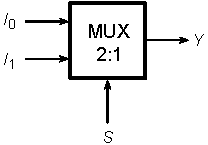
\includegraphics[height=.17\textheight]{mux21_sym}\hspace{4mm}
    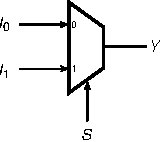
\includegraphics[height=.17\textheight]{mux21sym}\\[2mm]
    {\scriptsize Rectangular and funnel symbols}\\[2mm]
    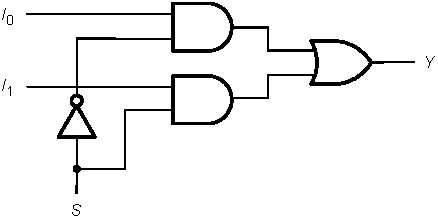
\includegraphics[width=.9\textwidth]{mux21_sch}
  \end{column}
  \begin{column}{.58\textwidth}
    \begin{itemize}\small\itemsep3pt
      \item A $2^n$:1 mux has $2^n$ data inputs, $n$ select lines and one output.
      \item $S = 0$: $Y = I_0$. $S = 1$: $Y = I_1$.
    \end{itemize}
    \centering\footnotesize\striped
    \begin{tabular}{@{}ccc|c@{}}
      \toprule
      $S$ & $I_1$ & $I_0$ & $Y$ \\
      \midrule
      0&0&0&0 \\ 0&0&1&1 \\ 0&1&0&0 \\ 0&1&1&1 \\
      1&0&0&0 \\ 1&0&1&0 \\ 1&1&0&1 \\ 1&1&1&1 \\
      \bottomrule
    \end{tabular}\\[1mm]
    {\small $Y = \overline{S}I_0 + SI_1$}
  \end{column}
  \end{columns}
\end{frame}

\begin{frame}{The 4:1 and 8:1 Multiplexers}
  \begin{columns}[c]
  \begin{column}{.45\textwidth}
    \centering
    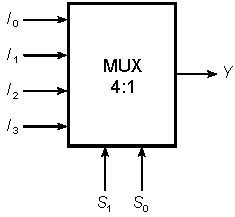
\includegraphics[height=.22\textheight]{mux41_sym}\\[2mm]
    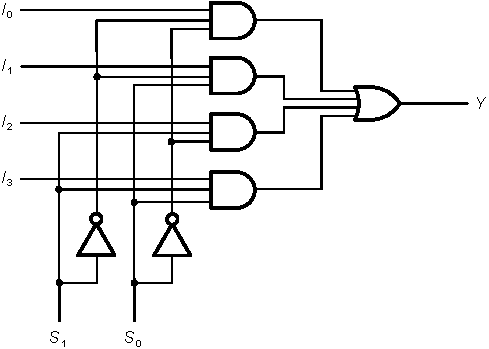
\includegraphics[height=.3\textheight]{mux41_sch}\\
    {\scriptsize 4 AND gates, 1 OR gate, 2 inverters}
  \end{column}
  \begin{column}{.53\textwidth}
    \centering\footnotesize\striped
    \begin{tabular}{@{}cc|c@{}}
      \toprule
      $S_1$ & $S_0$ & $Y$ \\
      \midrule
      0 & 0 & $I_0$ \\ 0 & 1 & $I_1$ \\ 1 & 0 & $I_2$ \\ 1 & 1 & $I_3$ \\
      \bottomrule
    \end{tabular}
    \small
    \[ Y = \overline{S_1}\,\overline{S_0}I_0 + \overline{S_1}S_0 I_1 + S_1\overline{S_0}I_2 + S_1S_0I_3 \]
    The 8:1 mux has eight such terms, one per data input, each ANDed with its select minterm.
  \end{column}
  \end{columns}
\end{frame}

%===============================================================================
\section{Multiplexer Applications}
%===============================================================================

\begin{frame}{Application: Data Selector}
  \centering
  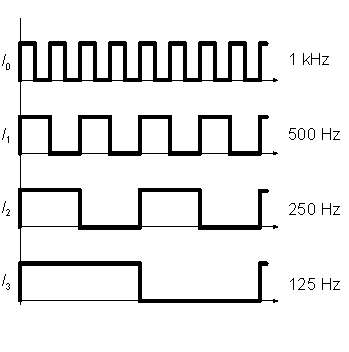
\includegraphics[height=.22\textheight]{mux41_waveselect1}\hspace{4mm}
  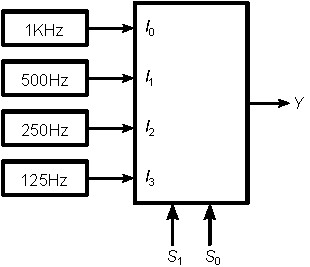
\includegraphics[height=.22\textheight]{mux41_waveselect2}\\[1mm]
  {\small Choosing one of four square waves of different frequencies}\\[2mm]
  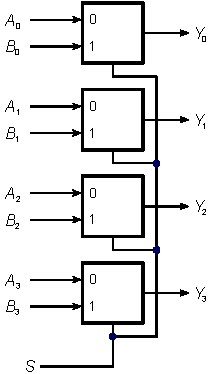
\includegraphics[height=.2\textheight]{mux21x4_sc}\hspace{2mm}$\Rightarrow$\hspace{2mm}
  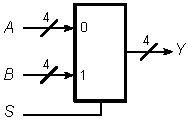
\includegraphics[height=.2\textheight]{mux21x4_tl}
  \begin{itemize}\small
    \item A set of four 2:1 muxes selects a whole nibble: $S = 0$ gives $Y = A$, $S = 1$ gives $Y = B$. This is a \alert{bus mux}.
  \end{itemize}
\end{frame}

\begin{frame}{Application: Implementing Boolean Functions}
  \begin{itemize}\small\itemsep3pt
    \item Any $n$-variable function can be realised with a $2^n$:1 mux. No minimisation is needed.
    \item Connect the variables to the select lines; set each data input to the function's truth-table value.
  \end{itemize}
  \begin{columns}[c]
  \begin{column}{.5\textwidth}
    \begin{block}{$Y = BC + A\overline{C}$ on an 8:1 mux}
      \small Minterms $m_3, m_4, m_6, m_7$. Set those data inputs to 1 and the rest to 0.
    \end{block}
    \centering\tiny\striped
    \begin{tabular}{@{}ccc|c@{}}
      \toprule
      $A$ & $B$ & $C$ & $Y$ \\
      \midrule
      0&0&0&0 \\ 0&0&1&0 \\ 0&1&0&0 \\ 0&1&1&1 \\
      1&0&0&1 \\ 1&0&1&0 \\ 1&1&0&1 \\ 1&1&1&1 \\
      \bottomrule
    \end{tabular}
  \end{column}
  \begin{column}{.48\textwidth}
    \centering
    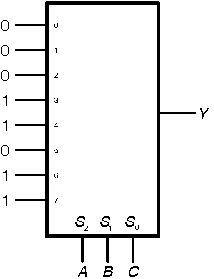
\includegraphics[height=.3\textheight]{mux81_lookup}\\
    {\scriptsize Gate-level: 4 gates. 8:1 mux: 12 gates, but no minimisation.}
  \end{column}
  \end{columns}
\end{frame}

\begin{frame}{Using a Smaller Mux}
  \begin{columns}[c]
  \begin{column}{.5\textwidth}
    \begin{itemize}\small\itemsep3pt
      \item $Y = BC + A\overline{C}$ on a 4:1 mux: $A, B$ drive $S_1, S_0$.
      \item For each $AB$ pair, $Y$ is $0$, $1$, $C$ or $\overline{C}$; connect that to the data input.
    \end{itemize}
    \centering\scriptsize\striped
    \begin{tabular}{@{}cccc|l@{}}
      \toprule
      $A$ & $B$ & $C$ & $Y$ & Mux input \\
      \midrule
      0&0&0&0 & \multirow{2}{*}{$I_0 = 0$} \\ 0&0&1&0 & \\
      0&1&0&0 & \multirow{2}{*}{$I_1 = C$} \\ 0&1&1&1 & \\
      1&0&0&1 & \multirow{2}{*}{$I_2 = \overline{C}$} \\ 1&0&1&0 & \\
      1&1&0&1 & \multirow{2}{*}{$I_3 = 1$} \\ 1&1&1&1 & \\
      \bottomrule
    \end{tabular}
  \end{column}
  \begin{column}{.48\textwidth}
    \centering
    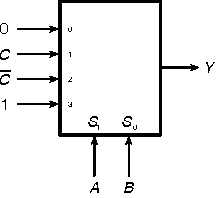
\includegraphics[width=.85\textwidth]{mux41_lookup}\\
    {\scriptsize 8 gates instead of 12.}
  \end{column}
  \end{columns}
\end{frame}

\begin{frame}{Basic Gates from a 2:1 Mux}
  \begin{columns}[t]
  \begin{column}{.32\textwidth}\centering
    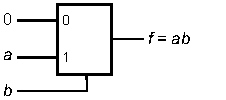
\includegraphics[width=.8\textwidth]{mux2and}\\[1mm]
    {\small AND: $f = \overline{b}(0) + b(a) = ab$}
  \end{column}
  \begin{column}{.32\textwidth}\centering
    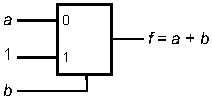
\includegraphics[width=.8\textwidth]{mux2or}\\[1mm]
    {\small OR: $f = \overline{b}(a) + b(1) = a + b$}
  \end{column}
  \begin{column}{.32\textwidth}\centering
    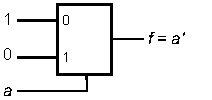
\includegraphics[width=.8\textwidth]{mux2inv}\\[1mm]
    {\small NOT: $f = \overline{a}(1) + a(0) = \overline{a}$}
  \end{column}
  \end{columns}
  \vspace{3mm}
  \begin{itemize}\small
    \item Mux-based implementation suits rapid design and FPGAs, where multiplexers are core building blocks. It is not the most efficient choice for simple functions.
  \end{itemize}
\end{frame}

%===============================================================================
\section{Demultiplexers}
%===============================================================================

\begin{frame}{Demultiplexers}
  \begin{columns}[c]
  \begin{column}{.5\textwidth}
    \begin{itemize}\small\itemsep3pt
      \item The opposite of a mux: one data input is routed to one of $2^n$ outputs chosen by $n$ select bits.
      \item A mux at the transmitter and a demux at the receiver let several sender-receiver pairs share one line.
    \end{itemize}
    \centering
    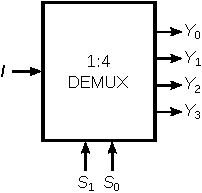
\includegraphics[height=.2\textheight]{demux14}\hspace{4mm}
    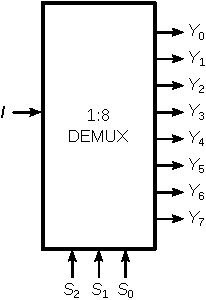
\includegraphics[height=.2\textheight]{demux18}\\
    {\scriptsize 1-to-4 and 1-to-8 demultiplexers}
  \end{column}
  \begin{column}{.48\textwidth}
    \centering
    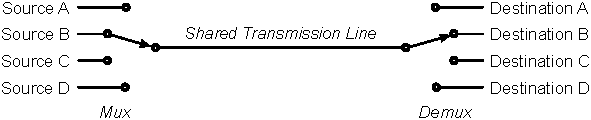
\includegraphics[width=\textwidth]{muxdemuxabstract}
  \end{column}
  \end{columns}
\end{frame}

%===============================================================================
\section{Decoders}
%===============================================================================

\begin{frame}{Decoders}
  \begin{columns}[c]
  \begin{column}{.5\textwidth}
    \begin{itemize}\small\itemsep3pt
      \item A decoder turns an input code into a code with more bits. The common type is the $n$-to-$2^n$ \alert{binary decoder}: the input value activates exactly one output.
      \item A calculator uses encoders on input and decoders on output.
    \end{itemize}
    \centering
    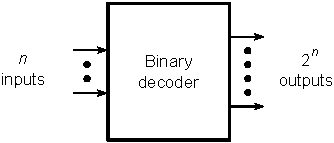
\includegraphics[width=.9\textwidth]{decoder_generic}
  \end{column}
  \begin{column}{.48\textwidth}
    \centering
    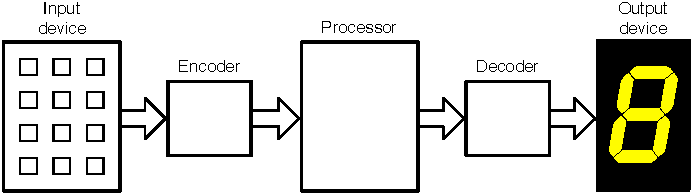
\includegraphics[width=\textwidth]{calculator}
  \end{column}
  \end{columns}
\end{frame}

\begin{frame}{The 2-to-4 Decoder}
  \begin{columns}[c]
  \begin{column}{.4\textwidth}
    \centering\footnotesize\striped
    \begin{tabular}{@{}cc|cccc@{}}
      \toprule
      $A$ & $B$ & $Y_0$ & $Y_1$ & $Y_2$ & $Y_3$ \\
      \midrule
      0&0&1&0&0&0 \\ 0&1&0&1&0&0 \\ 1&0&0&0&1&0 \\ 1&1&0&0&0&1 \\
      \bottomrule
    \end{tabular}\\[3mm]
    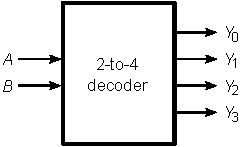
\includegraphics[width=.6\textwidth]{decoder2to4_sym}
  \end{column}
  \begin{column}{.58\textwidth}
    \centering
    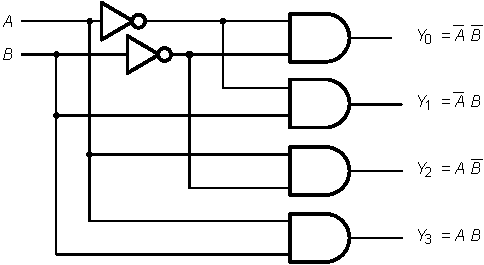
\includegraphics[width=.9\textwidth]{decoder2to4_sch}
    \begin{itemize}\small
      \item A 1-out-of-4 decoder produces all the minterms of two variables.
      \item The BCD-to-decimal decoder has 4 inputs and 10 outputs; inputs above 1001 disable all outputs.
    \end{itemize}
  \end{column}
  \end{columns}
\end{frame}

%===============================================================================
\section{Decoder Applications}
%===============================================================================

\begin{frame}{Decoder Applications}
  \begin{itemize}\small\itemsep4pt
    \item \alert{Address decoding}: select a device from the pattern on an address bus.
    \item \alert{Multiplexer control}: let one of many mux inputs through.
    \item \alert{Demultiplexer function}: send data from one input to one of many outputs.
    \item \alert{Implement a truth table directly}: a decoder produces all $2^n$ minterms, so an external OR gate forms any SOP function.
  \end{itemize}
  \begin{block}{Procedure}
    \small
    \begin{enumerate}\itemsep1pt
      \item Write the function as canonical SOP.
      \item Pick a decoder with as many inputs as the function has variables.
      \item OR together the outputs that match the function's minterms.
    \end{enumerate}
  \end{block}
\end{frame}

\begin{frame}{Example: Full Adder with a 3-to-8 Decoder}
  \begin{columns}[c]
  \begin{column}{.5\textwidth}
    \centering\scriptsize\striped
    \begin{tabular}{@{}ccc|cc@{}}
      \toprule
      $x$ & $y$ & $z$ & $s$ & $c$ \\
      \midrule
      0&0&0&0&0 \\ 0&0&1&1&0 \\ 0&1&0&1&0 \\ 0&1&1&0&1 \\
      1&0&0&1&0 \\ 1&0&1&0&1 \\ 1&1&0&0&1 \\ 1&1&1&1&1 \\
      \bottomrule
    \end{tabular}\\[2mm]
    \small $s = \sum m(1,2,4,7)$\\ $c = \sum m(3,5,6,7)$
  \end{column}
  \begin{column}{.48\textwidth}
    \centering
    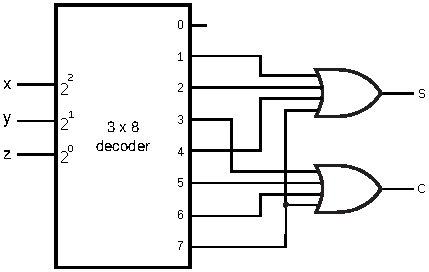
\includegraphics[width=\textwidth]{dec38fulladd}
  \end{column}
  \end{columns}
  \begin{itemize}\small
    \item OR decoder outputs 1, 2, 4, 7 for the sum and 3, 5, 6, 7 for the carry.
    \item If the decoder is built from NAND gates (active-low outputs), use NAND gates instead of OR (De Morgan).
  \end{itemize}
\end{frame}

%===============================================================================
\section{Seven-Segment Decoders}
%===============================================================================

\begin{frame}{Seven-Segment Displays}
  \begin{columns}[c]
  \begin{column}{.5\textwidth}
    \begin{itemize}\small\itemsep3pt
      \item Seven LED segments $a$ to $g$ (plus an optional decimal point) show the decimal digits.
      \item \alert{Common anode}: anodes tied together; a segment lights when its cathode is driven low.
      \item \alert{Common cathode}: cathodes tied together; a segment lights when its anode is driven high.
    \end{itemize}
    \centering
    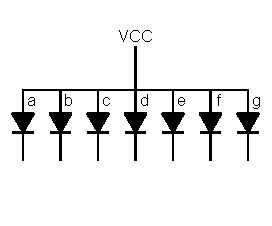
\includegraphics[height=.18\textheight]{commonanode}\hspace{4mm}
    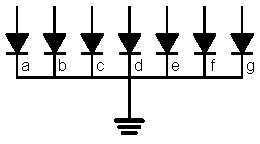
\includegraphics[height=.18\textheight]{commoncathode}
  \end{column}
  \begin{column}{.48\textwidth}
    \centering
    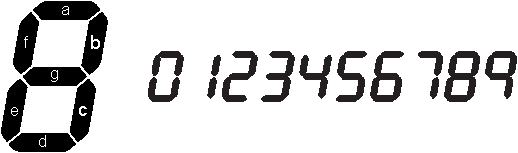
\includegraphics[width=\textwidth]{7segdisplay}
  \end{column}
  \end{columns}
\end{frame}

\begin{frame}{Common-Anode Segment Codes}
  \begin{columns}[c]
  \begin{column}{.55\textwidth}
    \centering\footnotesize\striped
    \begin{tabular}{@{}cc|ccccccc@{}}
      \toprule
      \textbf{Digit} & \textbf{BCD} & $a$ & $b$ & $c$ & $d$ & $e$ & $f$ & $g$ \\
      \midrule
      0 & 0000 & 0&0&0&0&0&0&1 \\
      1 & 0001 & 1&0&0&1&1&1&1 \\
      2 & 0010 & 0&0&1&0&0&1&0 \\
      3 & 0011 & 0&0&0&0&1&1&0 \\
      4 & 0100 & 1&0&0&1&1&0&0 \\
      5 & 0101 & 0&1&0&0&1&0&0 \\
      6 & 0110 & 0&1&0&0&0&0&0 \\
      7 & 0111 & 0&0&0&1&1&1&1 \\
      8 & 1000 & 0&0&0&0&0&0&0 \\
      9 & 1001 & 0&0&0&1&1&0&0 \\
      \bottomrule
    \end{tabular}
  \end{column}
  \begin{column}{.43\textwidth}
    \begin{itemize}\small\itemsep3pt
      \item Logic 0 turns a segment \alert{on}; logic 1 turns it off.
      \item Each segment output is a function of the four BCD inputs, so a BCD-to-7-segment decoder is a combinational design problem.
    \end{itemize}
  \end{column}
  \end{columns}
\end{frame}

\begin{frame}{7400-Family Decoder ICs}
  \centering\small\striped
  \begin{tabular}{@{}llll@{}}
    \toprule
    \textbf{Device} & \textbf{Function} & \textbf{Outputs} & \textbf{Key feature} \\
    \midrule
    74x138 & 3-to-8 decoder & Active-low & Three enable inputs \\
    74x139 & Dual 2-to-4 decoder & Active-low & Two independent channels \\
    74x42 & BCD-to-decimal & Active-low & 10 mutually exclusive outputs \\
    74x47 & BCD-to-7-segment & Active-low & Open-collector, common anode \\
    74x48 & BCD-to-7-segment & Active-high & Internal pull-ups, common cathode \\
    \bottomrule
  \end{tabular}
  \begin{itemize}\small
    \item Programmable logic and microcontrollers are alternatives, but these ICs remain useful for learning, driving displays and maintaining existing circuits.
    \item Check the datasheet: output circuitry and electrical characteristics differ.
  \end{itemize}
\end{frame}

\begin{frame}{The 74x47 Driver}
  \begin{columns}[c]
  \begin{column}{.3\textwidth}
    \centering
    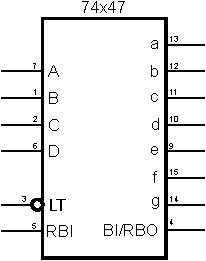
\includegraphics[width=.9\textwidth]{74x47_sym}\\[1mm]
    \scriptsize\striped
    \begin{tabular}{@{}ll@{}}
      LT & Lamp test \\
      RBI & Ripple blanking in \\
      RBO & Ripple blanking out \\
    \end{tabular}
  \end{column}
  \begin{column}{.68\textwidth}
    \centering
    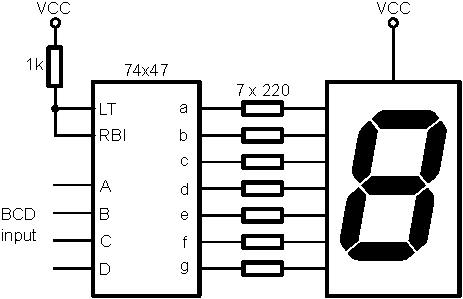
\includegraphics[width=.8\textwidth]{74x47_cir}
    \begin{itemize}\small\itemsep2pt
      \item For one digit: pull LT and RBI high. Never leave control inputs floating.
      \item Use a current-limiting resistor per segment, unless the display module has them.
    \end{itemize}
  \end{column}
  \end{columns}
\end{frame}

\begin{frame}{Leading-Zero Suppression}
  \centering
  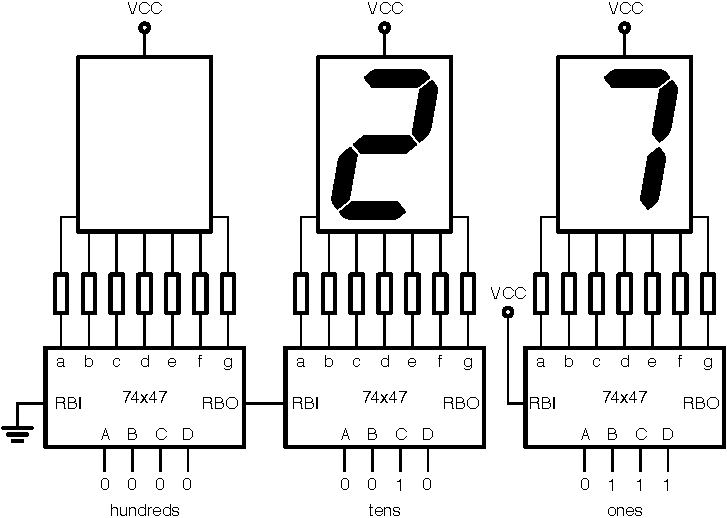
\includegraphics[height=.4\textheight]{74x47trio}
  \begin{itemize}\small\itemsep2pt
    \item When RBI is low and the BCD input is 0000, the decoder blanks the display and drives RBO low.
    \item Connect RBO of the hundreds digit to RBI of the tens digit, and RBO of the tens digit to RBI of the ones digit.
    \item Hold the hundreds RBI low (suppress) and the ones RBI high, so at least one digit always shows.
  \end{itemize}
\end{frame}

%===============================================================================
\section{Encoders}
%===============================================================================

\begin{frame}{Encoders}
  \begin{columns}[c]
  \begin{column}{.4\textwidth}
    \centering
    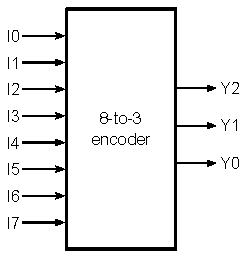
\includegraphics[height=.22\textheight]{enc8x3_tl}
  \end{column}
  \begin{column}{.58\textwidth}
    \begin{itemize}\small\itemsep3pt
      \item The opposite of a decoder: $2^n$ input lines are compressed into an $n$-bit code.
      \item An 8-to-3 encoder outputs the binary index of the single active input.
      \item In an ideal encoder, only \alert{one} input may be active at a time.
    \end{itemize}
  \end{column}
  \end{columns}
  \centering\scriptsize\striped
  \begin{tabular}{@{}cccccccc|ccc@{}}
    \toprule
    $I_0$&$I_1$&$I_2$&$I_3$&$I_4$&$I_5$&$I_6$&$I_7$&$Y_2$&$Y_1$&$Y_0$ \\
    \midrule
    1&0&0&0&0&0&0&0&0&0&0 \\ 0&1&0&0&0&0&0&0&0&0&1 \\ 0&0&1&0&0&0&0&0&0&1&0 \\ 0&0&0&1&0&0&0&0&0&1&1 \\
    0&0&0&0&1&0&0&0&1&0&0 \\ 0&0&0&0&0&1&0&0&1&0&1 \\ 0&0&0&0&0&0&1&0&1&1&0 \\ 0&0&0&0&0&0&0&1&1&1&1 \\
    \bottomrule
  \end{tabular}
\end{frame}

\begin{frame}{Priority Encoders}
  \begin{columns}[c]
  \begin{column}{.5\textwidth}
    \begin{itemize}\small\itemsep3pt
      \item If several inputs can be active together, a plain encoder gives undefined results.
      \item A \alert{priority encoder} considers only the highest-priority active input.
      \item Used where many devices may ask for attention at once but only one is served at a time.
    \end{itemize}
  \end{column}
  \begin{column}{.48\textwidth}
    \centering\tiny\striped
    \begin{tabular}{@{}cccccccc|ccc@{}}
      \toprule
      $I_0$&$I_1$&$I_2$&$I_3$&$I_4$&$I_5$&$I_6$&$I_7$&$Y_2$&$Y_1$&$Y_0$ \\
      \midrule
      1&0&0&0&0&0&0&0&0&0&0 \\
      $\times$&1&0&0&0&0&0&0&0&0&1 \\
      $\times$&$\times$&1&0&0&0&0&0&0&1&0 \\
      $\times$&$\times$&$\times$&1&0&0&0&0&0&1&1 \\
      $\times$&$\times$&$\times$&$\times$&1&0&0&0&1&0&0 \\
      $\times$&$\times$&$\times$&$\times$&$\times$&1&0&0&1&0&1 \\
      $\times$&$\times$&$\times$&$\times$&$\times$&$\times$&1&0&1&1&0 \\
      $\times$&$\times$&$\times$&$\times$&$\times$&$\times$&$\times$&1&1&1&1 \\
      \bottomrule
    \end{tabular}
  \end{column}
  \end{columns}
\end{frame}

%===============================================================================
\section{Buffers as Multiplexers}
%===============================================================================

\begin{frame}{Tri-State Buffers as a Mux}
  \begin{columns}[c]
  \begin{column}{.5\textwidth}
    \begin{itemize}\small\itemsep3pt
      \item Each tri-state buffer has an enable: on, it drives the bus; off, it is high impedance (disconnected).
      \item With exactly one buffer enabled, the bus carries one source: a mux at the wire level.
      \item A \alert{decoder} makes the enables, so at most one buffer drives the bus. This prevents contention and short circuits.
    \end{itemize}
  \end{column}
  \begin{column}{.48\textwidth}
    \centering
    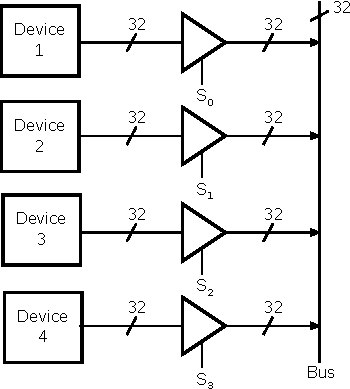
\includegraphics[height=.55\textheight]{tristate32}
  \end{column}
  \end{columns}
\end{frame}

\begin{frame}{Back to the Opening Question}
  \begin{block}{A 3-input function with no gates}
    \small An \alert{8:1 multiplexer}. Wire the three inputs to the select lines and hard-wire each data input to the truth-table value (0 or 1). Any 3-variable function works, so 8:1 is the smallest mux that \emph{always} works.\\[2mm]
    With a little more care (using $C$ or $\overline{C}$ on the data inputs) a 4:1 mux can implement many of them too.
  \end{block}
\end{frame}

%===============================================================================
\section{Summary}
%===============================================================================

\begin{frame}{Summary}
  \begin{itemize}\itemsep3pt\small
    \item A $2^n$:1 mux selects one of $2^n$ inputs with $n$ select bits; a demux routes one input to one of $2^n$ outputs.
    \item A decoder asserts exactly one of $2^n$ outputs: a one-hot translator.
    \item A $2^n$:1 mux can implement \alert{any} $n$-variable function by wiring its data inputs to the truth-table values.
    \item A priority encoder returns the index of the highest-priority active input; a plain encoder needs at most one active input.
    \item Tri-state buffers on a shared bus form a multi-source mux; only one driver may be enabled at a time.
  \end{itemize}
  \begin{block}{Looking ahead}
    Chapter 9 shows how arithmetic circuits combine bits to calculate sums, differences and comparisons.
  \end{block}
\end{frame}

\end{document}
